%%%%%%%%%%%%%%%%%%%%%%%%%%%%%%%%%%%%%%%%%%%%%%%%%%%%%%%%%%%%%%%%%
%
% Project     : Turnverein App
% Title       : 
% File        : umsetzung.tex Rev. 00
% Date        : 07.07.14
% Author      : Raffael Santschi
%
%%%%%%%%%%%%%%%%%%%%%%%%%%%%%%%%%%%%%%%%%%%%%%%%%%%%%%%%%%%%%%%%%

\chapter{Umsetzung des Prototyps}\label{chap.umsetzung}
In diesem Kapitel wird kurz auf die Entwicklungsumgebung, die für dieses Projekt verwendet wurde, eingegangen. Danach wird erklärt, wie die Umsetzung des Backends und des Mobile App Prototyps durchgeführt wurde.

\section{Entwicklungsumgebung}\label{entwicklungsumgebung}
Ein Softwareprojekt benötigt immer eine gewisse Umgebung, welche die erforderlichen Funktionen erfüllt. Die Entwicklung einer App mit Hilfe von Phonegap kommt mit wenig aus und die Entwicklungsumgebung ist schnell aufgebaut.

\subsection{IDE - Integrated Development Environment}
Eine IDE, um welche man sicher nicht herum kommt, ist XCode. Sie wird benötigt um die App zu paketieren und sie direkt zur Analyse von Apple hochzuladen. Zusätzlich wurde noch Aptana Studio, welches für Webentwicklung ausgelegt ist, verwendet. Hier könnte man aber auf beliebige Alternativen umsteigen und notfalls auch mit einem gewöhnlichen Texteditor arbeiten. Die Vorteile einer IDE sind Syntax-Highlighting, -Checking und Autocompletion.

\begin{figure}[h]
\centering
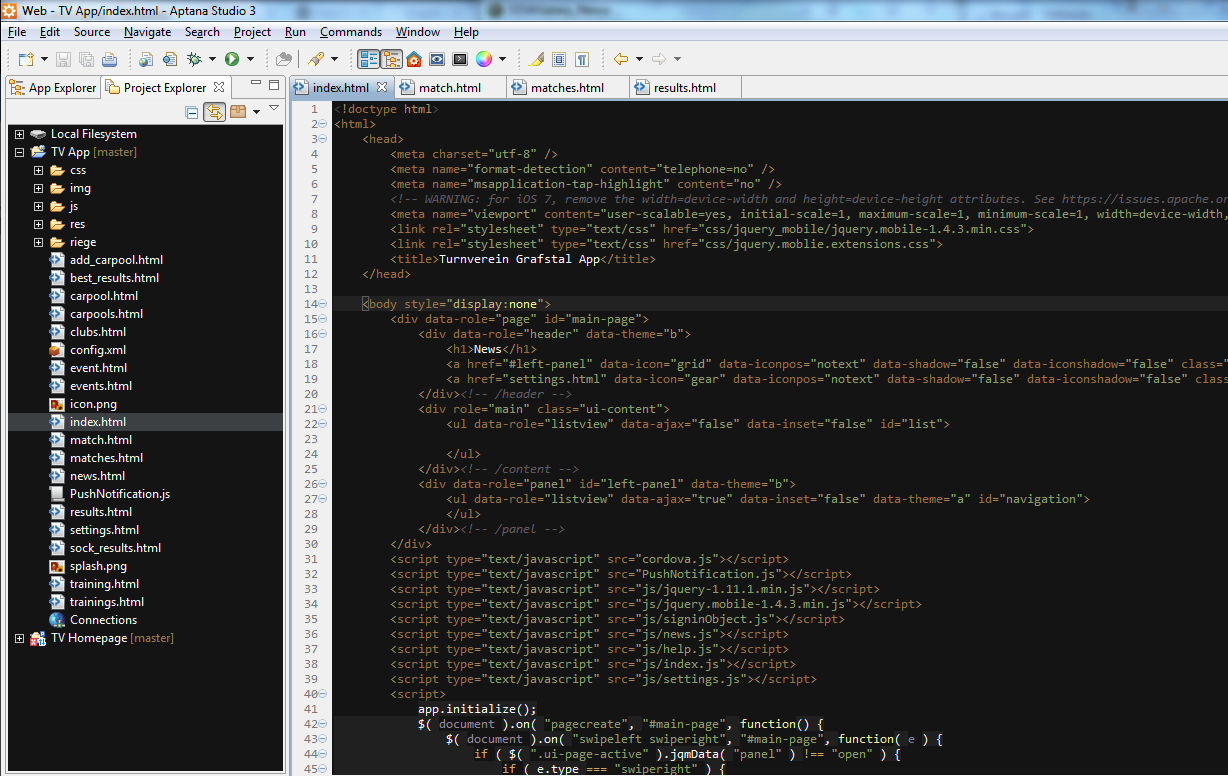
\includegraphics[scale=0.5]{images/aptana.png}
\caption{Aptana Studio}
\label{fig:aptana}
\end{figure}


\subsection{Versionierung}
Versionieriung ist in der Softwareentwicklung ein sehr wichtiges Thema, früher war das ein manueller Task, heute gibt es verschiedenste Tools, die einen dabei unterstützen. In diesem Projekt wurde git (siehe \cite{git}) verwendet, was eines der verbreitetsten Versionierungstools ist. Das Remote Repository wurde auf Github (siehe \cite{github_app}) erstellt. Es wurde geschaut, dass der Code jeden Abend auf das Repository geladen wurde, damit man auch gleich ein Backup hat.

\begin{figure}[h]
\centering
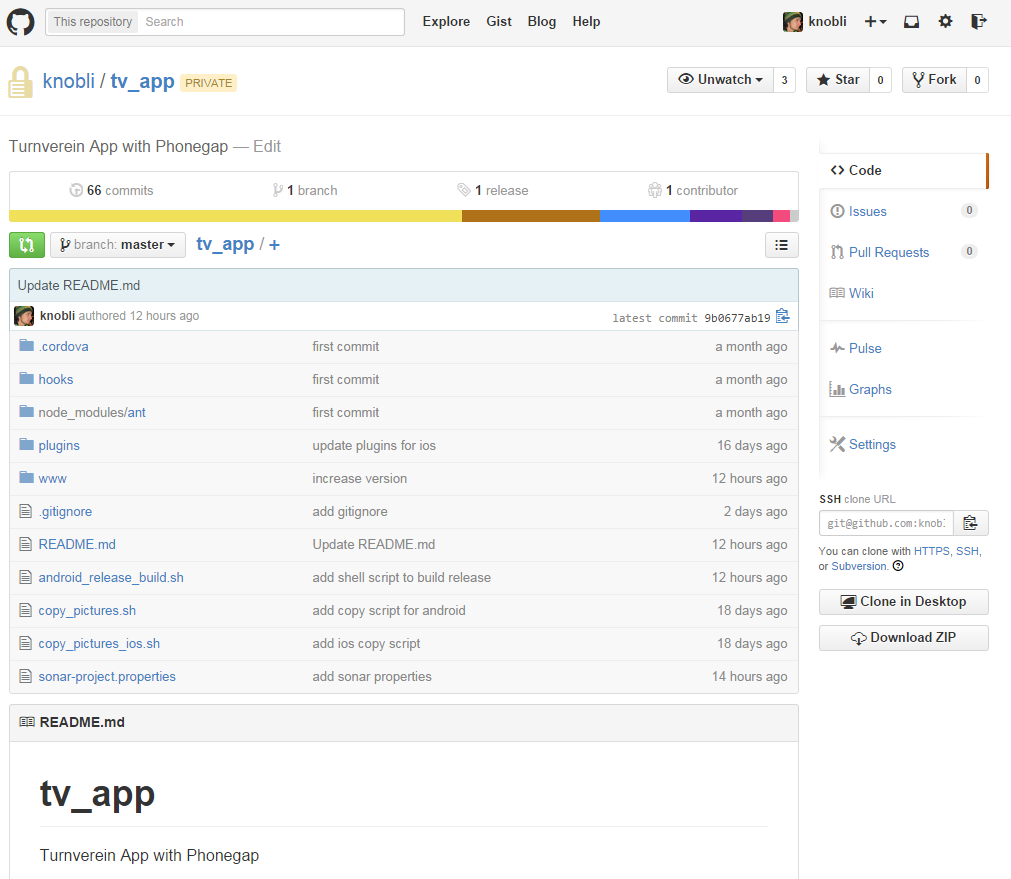
\includegraphics[scale=0.5]{images/github.png}
\caption{Github Repository}
\label{fig:github_repo}
\end{figure}

\newpage
\subsection{SDK - Software Development Kit}
Für die Entwicklung der App auf den beiden Plattformen Android und iOS wurden die dazugehörigen SDKs gebraucht, um die Applikation in einem Emulator laufen zu lassen. Vor allem bei Android, mit seinen diversen Gerätevariationen, macht das Sinn, weil man mit dem Emulator jedes beliebige Device emulieren kann.

\begin{figure}[h]
\centering
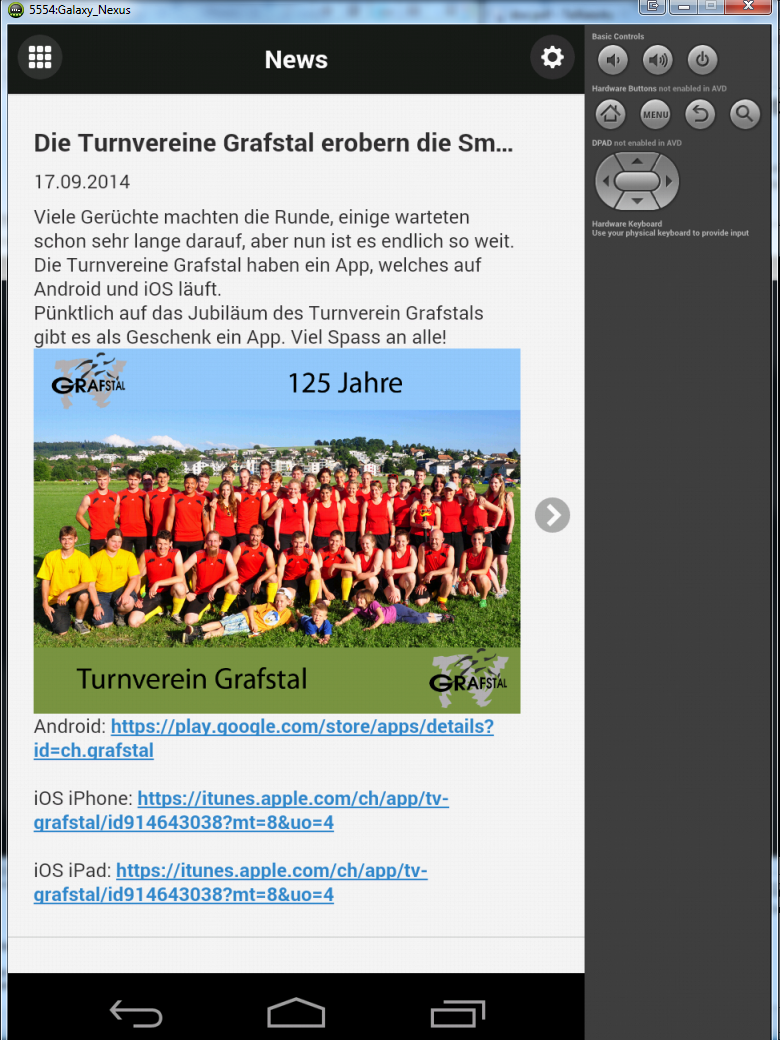
\includegraphics[scale=0.25]{images/android_emulator.png}
\caption{Android Emulator}
\label{fig:android_emulator}
\end{figure}

\FloatBarrier
\subsection{Webbrowser}
Die App wurde nicht nur auf Emulatoren getestet, sondern auch in Browsern. Dazu wurde auf Windows mit Google Chrome und auf Mac OSX mit Safari gearbeitet.

\subsection{Technische Geräte}
Push-Nachrichten können weder auf Emulatoren noch in Webbrowsern getestet werden, dafür benötigt man ein physisches Gerät. Die App wurde auf einem iPhone 4S, iPhone 5S, iPad und Samsung Ace getestet. Für die Entwicklung wurde ein Windows PC verwendet. Damit XCode benutzt werden konnte, wurde zusätzlich noch auf einem iMac gearbeitet.

\newpage
\subsection{Testen - Analysieren}
Zusätzlich zu den manuellen Tests an Geräten und  Emulatoren wurden auch automatisierte Tests und Analysen durchgeführt. Für die automatisierten Tests im Backend wurde PHPunit (siehe \cite{phpunit}) verwendet und für die statische Code Analyse wurde Sonar (siehe \cite{sonar}) mit dem PHP und Web Plugin (siehe Abbildung \ref{fig:sonar_backend} und \ref{fig:sonar_app}) aufgesetzt und verwendet. Damit das API direkt getestet werden konnte, wurde die Chrome App 'Advanced REST client' (siehe Abbildung \ref{fig:advanced_rest_client}) verwendet.

\begin{figure}[h]
\centering
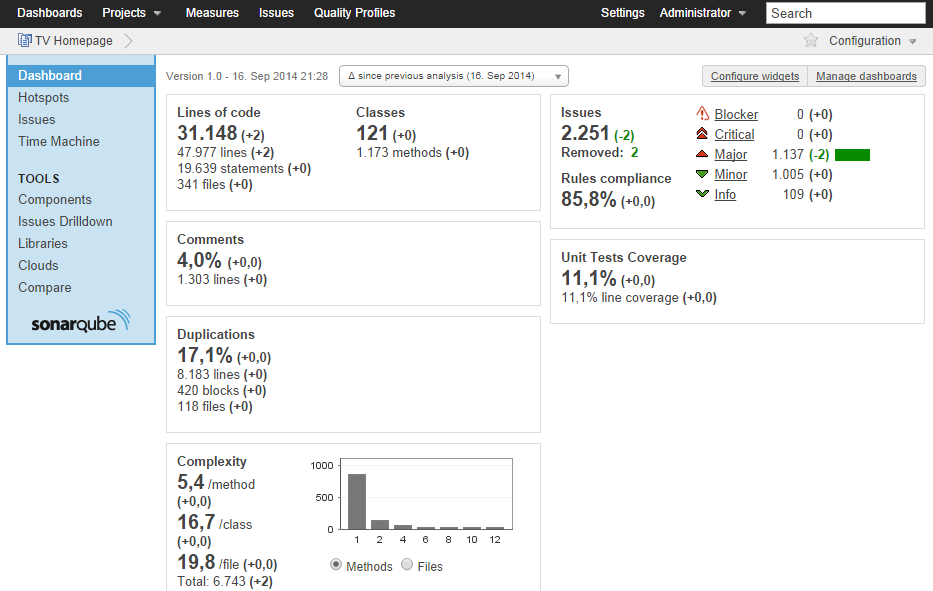
\includegraphics[scale=0.5]{images/sonar_backend.png}
\caption{Sonar - statische Code Analyse Backend}
\label{fig:sonar_backend}
\end{figure}

\begin{figure}[h]
\centering
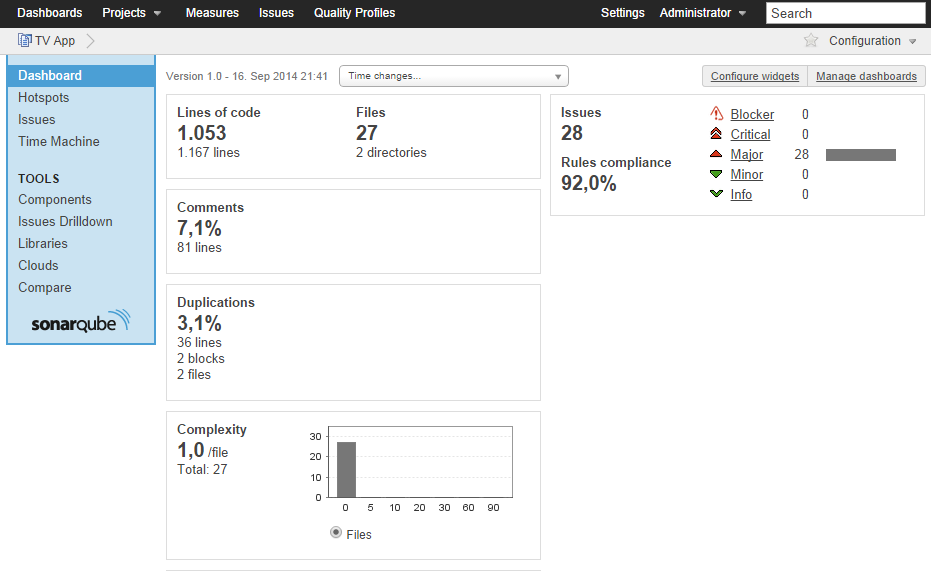
\includegraphics[scale=0.5]{images/sonar_app.png}
\caption{Sonar - statische Code Analyse App}
\label{fig:sonar_app}
\end{figure}

\begin{figure}[h]
\centering
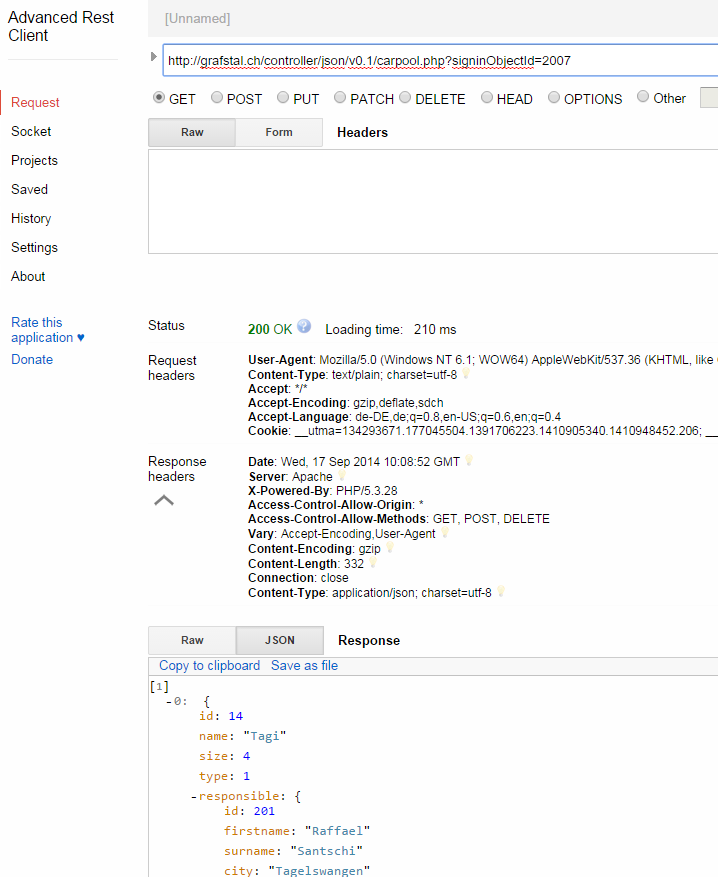
\includegraphics[scale=0.5]{images/advanced_rest_client.png}
\caption{Advanced Rest client}
\label{fig:advanced_rest_client}
\end{figure}

\FloatBarrier


\clearpage
\section{Backend}\label{impl_backend}
In diesem Unterkapitel werden das Refactoring des Backends beschrieben und eine Übersicht der Push-Nachricht Implementierung vermittelt.

\subsection{Refactoring}
In diesem Unterkapitel wird kurz der vorgefundene Ist-Zustand beschrieben und danach die Schritte, welche unternommen wurden, um das Backend wartbarer und flexibler zu machen.

\subsubsection{Ist-Zustand}
Am Anfang dieses Projekts war in jeder Klasse HTML- mit PHP-Code vermischt und SQL-Abfragen waren überall verstreut. Dies machte es schwierig den Code zu warten. Zusätzlich wurde jede save-, update-, load- und delete-Anweisung von Objekten, wenn es denn solche gab, selber implementiert, was sehr mühsam und unflexibel war. Zudem erweiterten ähnliche Objekte zwar eine Super-Klasse, teilten sich aber keine Tabelle und hatten somit auch verschiedene ID-Sequenzen.\\

Schnell wurde klar, dass man mit diesem Stand kein API aufbauen sollte, welches dann von der App angesprochen wird. Um den Code besser zu strukturieren, übersichtlicher und vor allem auch testbar zu machen, wurde ein Refactoring (siehe \cite{feathers2004working}) durchgeführt. Ausgehend von der Strategie für das Refactoring wurde Doctrine in das Projekt eingebunden. Doctrine ist, wie schon im Kapitel \ref{arch_backend} erklärt, ein ORM, welches, richtig eingesetzt, viel Arbeit abnehmen kann. Damit man Doctrine jedoch sinnvoll verwenden konnte, benötigte es zuerst einige Zeit für die Analyse und die Umstellungen.

\subsubsection{Refactoring}
Zuerst wurde geschaut, was zusammengefasst werden konnte. Alle Entities, bei denen man sich anmelden kann, wurden ganz getreu dem 'Don’t repeat yourself' Prinzip als SigninObject zusammengefasst, da sie sehr viele gleiche Attribute und Funkionen haben. Im gleichen Zug wurde die Datenbank normalisiert, da zum Teil gleiche Ortsnamen in verschiedenen Tabellen vorhanden waren. Da die einzelnen Typen jedoch auch spezifische Attribute haben, wurde eine Joined-Inheritance (siehe \cite{inheritance_java} und \cite{inheritance_doctrine}) angewendet, welche von vielen ORMs unterstützt wird. Die Joined-Inheritance basiert auf einer Grundtabelle, welche alle gemeinsamen Attribute beinhaltet und einer spezifischen Tabelle, welche die anderen Attribute beinhaltet. Die Tabellen werden über eine DiscriminatorColumn miteinander verknüpft. In diesem Konstrukt wurde auch ein Strategy-Pattern (siehe \cite{gof_book}) verwendet, um verschiedene Informationen im Kalender\footnote{Der Kalender (nicht in diesem Projekt entwickelt) kann über ein ics-File auf Geräten eingebunden werden.} anzuzeigen.\\

Dieser Umbau hat den grossen Vorteil, dass für jeden Veranstaltungstyp, sei das ein Training, Match, Sitzung, Anlass oder Helfereinsatz, die gleiche Anmeldefunkion verwendet werden kann. Der Umbau machte sich auch bei der Entwicklung der Fahrgemeinschaftsverwaltung bezahlt, da diese nur ein mal implementiert werden musste.\\

\begin{figure}[h]
\centering
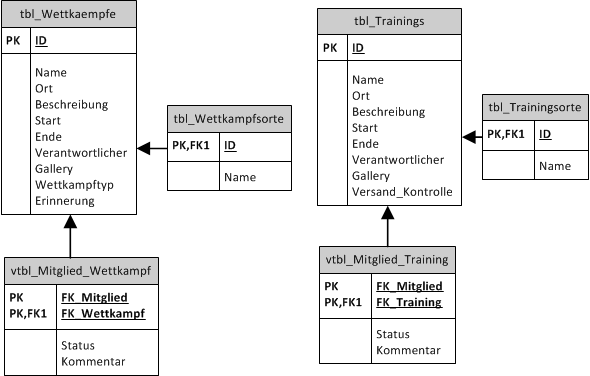
\includegraphics[scale=0.7]{images/visio/datenbankdiagramm_alt.png}
\caption{Datenbankdiagramm alt}
\label{fig:db_schema_alt}
\end{figure}

Das Datenbankdiagramm (siehe Abbildung \ref{fig:db_schema_alt}) zeigt einen kleinen Ausschnitt aus dem Datenbank Schema von früher. Jeder Veranstaltungstyp hatte seine eigene Ortstabelle und seine eigene Verknüpfungstabelle für die Anmeldungen. Wenn man sich nun vorstellt, dass dieses Konstrukt für die fünf verschiedenen Typen vorhanden war, kann man sich denken, wie viele Tabellen schon bereits nur für die Anmeldungen vorhanden waren. Nach dem Refactoring sah das Datenbankdiagramm (siehe Abbildung \ref{fig:db_schema_neu}) etwas einfacher aus. Die Orte waren nun in einer Tabelle, die Anmeldungen auch und alle gemeinsamen Attribute wurden in der TerminObjekte-Tabelle gespeichert.

\begin{figure}[h]
\centering
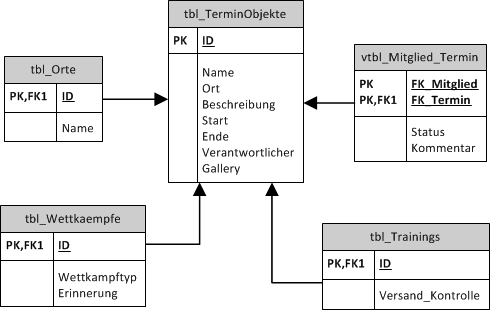
\includegraphics[scale=0.7]{images/visio/datenbankdiagramm_neu.png}
\caption{Datenbankdiagramm neu}
\label{fig:db_schema_neu}
\end{figure}

\FloatBarrier
Durch das Refactoring werden weniger SQL-Statements direkt in den Webseiten abgesetzt. Es wird vermehrt\footnote{Nur an Orten, wo die Objekte innerhalb dieses Projektes angefasst wurden} mit Objekten gearbeitet. Ein Repository liefert die gewünschten Objekte zur Webseite, die Abfrage Logik ist somit zentralisiert. Das Repository arbeitet mit einer Object Query Language (OQL), bei welcher man nicht über die Spalten der Tabelle Werte abfragt, sondern über Attribute des Objekts. Eine Änderung des Spaltennamens hat somit keine grössere Auswirkung als eine kleine Änderung in der Entity.\\

Die Struktur sieht nach der Implementierung von Doctrine wie folgt aus:
\begin{itemize}
\item Entity: Attribute, Getter und Setter
\item Enity-Manager: speichert, löscht und lädt Entities oder gibt das Repository der Entity zurück
\item Repository: spezifische Abfrage-Logik
\item Services\footnote{Services werden nicht von Doctrine vorgegeben, wurden aber als eine weitere Schicht sogenannte Verarbeitungsschicht implementiert}: Business-Logik
\end{itemize}

\newpage
\subsubsection{Facts and Figures}
Das Refactoring war zwar sehr zeitaufwendig, hat jedoch bei einigen Implementationen die Komplexität stark reduziert, Zeitersparnisse eingebracht und wird auch in Zukunft vieles erleichtern.
\begin{itemize}
\item Testabdeckung: Das Testen stellte sich vorher als extrem schwierig heraus und ist nun mit den Kapselungen viel einfacher. Es konnte während des Projekts doch immerhin eine Testabdeckung von 11.1\% erreicht werden. Dieses Resultat wird natürlich noch sehr verfälscht durch Seiten und Funktionen, welche nicht Teil dieses Projekts waren.
\item Duplikate: Der Prozentsatz der duplizierten Linien konnte um fast 6\% reduziert werden, was etwa 4'000 Lines of code bedeutet.
\item Komplexität: Die Komplexität pro Klasse konnte von 40 auf 17 gesenkt werden.
\item Rule compliance: Die Rule compliance konnte um knapp 7\% gesteigert werden.
\item Issues: Über 3000 Issues, darunter alle kritischen und Blocker Issues, konnten behoben werden.
\end{itemize}


\subsection{Push-Nachrichten}
Das Versenden von Push-Nachrichten funktioniert bei iOS und Android ähnlich, jedoch sind die Vorbedingungen sehr unterschiedlich. Bei Android wird ein API-Key verwendet, welchen man in der Google Developers Console erstellen kann. Dazu muss man ein Projekt erstellen und 'Google Cloud Messaging for Android' aktivieren. Nun kann man einen neuen API-Key erstellen, welcher dann im Backend benötigt wird. Die Projektnummer ist zugleich die Sender ID und wird bei der Registrierung des produktiven Apps über Phonegap benötigt. (siehe dazu \cite{android_push_android} und \cite{devgirl_push_android})\\


Bei iOS ist das etwas anders, als erstes braucht man ein Zertifikat, da nur ein Server mit diesem Zertifikat Push-Nachrichten an den APNS senden darf. Es gibt ein Zertifikat für den Entwicklungsserver und ein weiteres für den produktiven Server. Über den Entwicklungsserver können nur verknüpfte\footnote{um die App auf einem Gerät zu testen, muss man es zuerst mit dem Developer Account verknüpfen} Geräte im Entwicklungsmodus erreicht werden. Zusätzlich muss für das Testen der Push-Nachrichten noch ein iOS App Development Provisioning Profile erstellt werden, welches dann auch mit dem Developer Account und den Test Geräten verknüpft wird. Bei der Erstellung der Zertifikate ist es wichtig, dass die App ID mit dem Projekt übereinstimmt, ansonsten kommen die Push-Nachrichten nicht an. Die Registrierung des produktiven Apps über Phonegap ist ganz einfach und nicht projektspezifisch. (siehe dazu \cite{ios_push})\\

Nach der Registrierung des jeweiligen Services schickt die App den Geräteschlüssel mit der Mitglieder ID ans Backend, welches den Schlüssel mit der Verknüpfung zum Mitglied speichert. Nun hat man den Schlüssel, den man für das gezielte Versenden von Push-Nachrichten benötigt.
\begin{figure}[ht]
\centering
\subfigure[Registration]{
  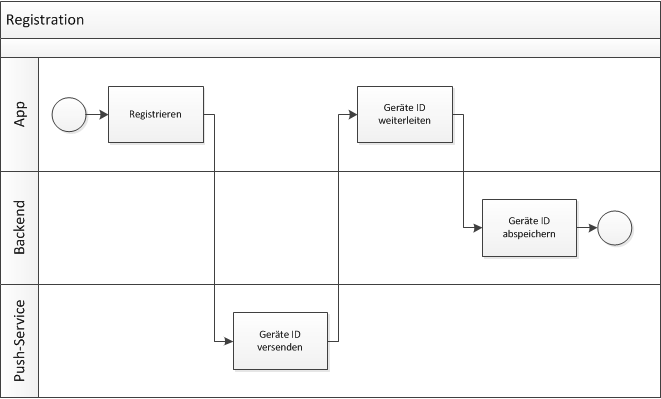
\includegraphics[scale=0.7]{images/visio/push_notification_flow_reg.png}
  \label{fig:push_notification_flow_reg}
}
\subfigure[Mitteilung versenden]{
  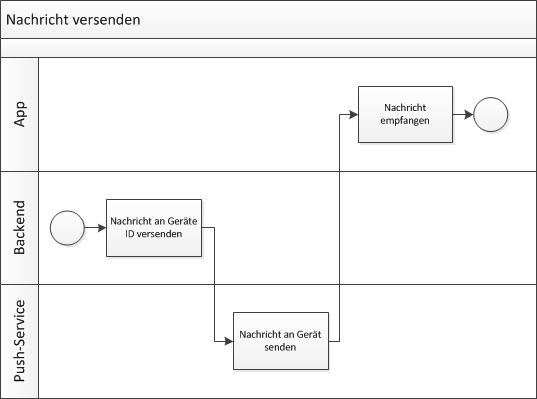
\includegraphics[scale=0.7]{images/visio/push_notification_flow_send.png}
  \label{fig:push_notification_flow_send}
}
\label{fig:app_settings}
\caption{Ablauf von Push-Nachrichten}
\end{figure}

\subsection{Resultierende Quellcode}
Dieses Projekt wurde auf einem bereits bestehenden Backend aufgebaut, alle Änderungen ab der Revision 3c54a42a698abdeee1779c71542786bd6707237b wurden innerhalb dieses Projekt getätigt. Für die Arbeiten im Refactoring wurden zwei neue Branches erstellt. Zum einen der 'refactoring' Branch, in welchem die Änderungen für die Datenmigration abgelegt wurden und zum anderen der 'jpa\_implementation' Branch, in welchem das eigentliche Refactoring durchgeführt wurde. In diesem Branch wurde gearbeitet bis der Stand produktionsreif war. Der 'jpa\_implementation' Branch wurde dann wieder in den 'master' Branch geführt. In der Projektzeit 


\section{Mobile App}\label{impl_moblie_app}
In diesem Unterkapitel werden neben einem detailierten Aufbau der App, die unterschiedlichen Provisioning Prozesse und die Probleme bei der Umsetzung beschrieben.

\subsection{Aufbau}
Das Menü (siehe Abbildung \ref{fig:navigation}) der App wurde sehr schlicht gehalten und sehr leicht erweiterbar gemacht. Die Einträge News, Vereine und Veranstaltungen sind für alle Benutzer sichtbar, wenn auch mit benutzerspezifischem Inhalt und Design. Der Link zu den Resultaten ist nur für angemeldete Benutzer verfügbar.

\begin{figure}[h]
\centering
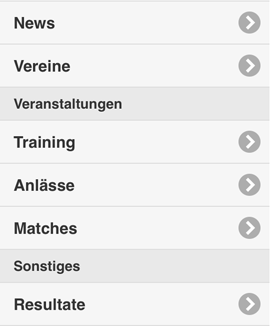
\includegraphics{images/app/navigation.png}
\caption{Navigation im App}
\label{fig:navigation}
\end{figure}

\FloatBarrier
\subsubsection{News}
Die News Seite (siehe Abbildung \ref{fig:app_news}) ist zugleich auch die Startseite, wenn die App aufgemacht wird. Auf ihr werden die neusten drei Berichte angezeigt. Der Aufbau ist wie auf der Homepage, die Elemente enthalten lediglich einen Einleitungstext. Erst wenn man auf das Element klickt kann man den ganzen Bericht lesen. Dies hat den einfachen Grund, dass die Berichte zum Teil sehr lang sind und dann die anderen Berichte verloren gehen. Bei angemeldeten Mitgliedern wird zusätzlich noch die nächste Veranstaltung angezeigt, damit man sich sofort an- bzw. abmelden und wichtige Informationen nachschlagen kann.

\begin{figure}[h]
\centering

\includegraphics[scale=0.5]{images/app/news.png}
\caption{News Seite}
\label{fig:app_news}
\end{figure}

\FloatBarrier
\subsubsection{Vereine}
Die Vereine Seite (siehe Abbildung \ref{fig:app_vereine})  listet alle Vereine und Riegen der Turner Familie Grafstal auf. Wenn man auf eine Riege klickt, erhält man zusätzliche Informationen, wie zum Beispiel die Trainingszeiten. Diese Seite enthält vor allem Informationen für die Öffentlichkeit oder ist ein Nachschlagewerk für Mitglieder.


\begin{figure}[h]
\centering
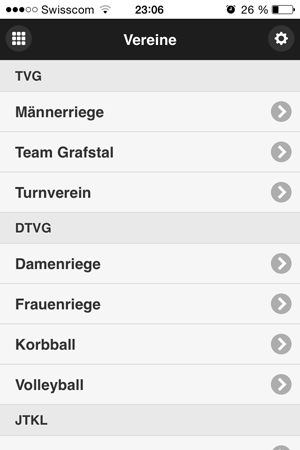
\includegraphics[scale=0.5]{images/app/vereine.png}
\caption{Vereinsseite}
\label{fig:app_vereine}
\end{figure}

\newpage
\FloatBarrier
\subsubsection{Veranstaltungen}
Die drei Veranstaltungsseiten sind alle gleich aufgebaut (siehe Abbildung \ref{fig:app_trainings}), sie zeigen die aktuellen Elemente mit Name, Datum, Zeit, Ort und Verantwortlichen. Falls der Benutzer angemeldet ist, wird durch Farbe angezeigt, ob er sich angemeldet (grün), abgemeldet (rot) oder nichts von beidem (grau) hat.
\begin{figure}[ht]
\centering
\subfigure[Anlässe (nicht angemeldet)]{
  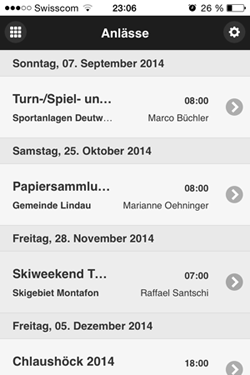
\includegraphics[scale=0.5]{images/app/events.png}
  \label{fig:app_events}
}
\subfigure[Trainings (angemeldet)]{
  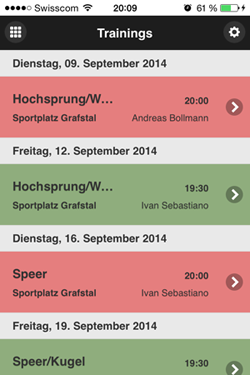
\includegraphics[scale=0.5]{images/app/trainings.png}
  \label{fig:app_trainings}
}
\label{fig:app_singinobjects}
\caption{Veranstaltungen}
\end{figure}

Wenn auf eine Veranstaltung geklickt wird, geht eine Detailansicht (siehe Abbildung \ref{fig:app_detail_event}) auf. In dieser Ansicht erhält man weitere Information, kann sich an- und abmelden und kommt auch zu den Fahrgemeinschaften. Die Information, wer sich angemeldet hat, sehen nur angemeldete Benutzer.

\begin{figure}[h]
\centering
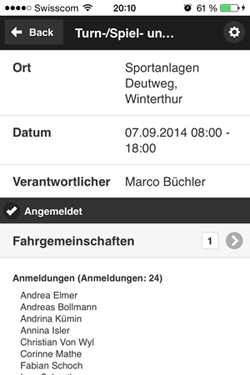
\includegraphics[scale=0.5]{images/app/event_detail.png}
\caption{Anlass Details}
\label{fig:app_detail_event}
\end{figure}

\newpage
\FloatBarrier
\subsubsection{Fahrgemeinschaften}
Bei jeder Veranstaltung können Fahrgemeinschaften erstellt werden, welche dann in der Übersicht (siehe Abbildung \ref{fig:app_carpools}) angezeigt werden. Man sieht den Namen, den Fahrer und dessen Wohnort. Zusätzlich sieht man, wie viele Plätze noch frei sind oder ob man bereits angemeldet ist. In der Detailansicht (siehe Abbildung \ref{fig:app_carpool_detail}) kann man sich anmelden und erhält eine Liste der Mitfahrenden.
\begin{figure}[ht]
\centering
\subfigure[Fahrgemeinschaften]{
  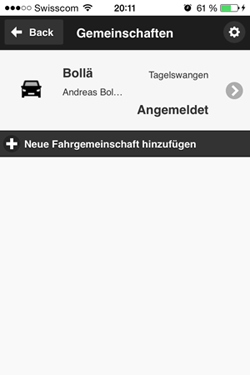
\includegraphics[scale=0.5]{images/app/carpools.png}
  \label{fig:app_carpools}
}
\subfigure[Fahrgemeinschaft Detail]{
  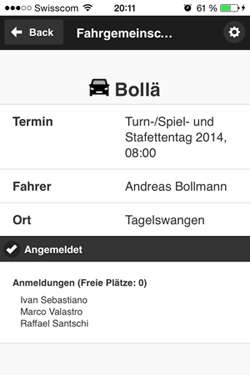
\includegraphics[scale=0.5]{images/app/carpool_detail.png}
  \label{fig:app_carpool_detail}
}
\label{fig:app_carpool_page}
\caption{Veranstaltungen}
\end{figure}

Im Formular (siehe Abbildung \ref{fig:app_add_carpool}) für die Erstellung einer neuen Fahrgemeinschaft muss man einen Namen angeben und kann den Typ der Gemeinschaft wählen, nur wenn es eine 'Car'-Fahrgemeinschaft ist, muss man die freien Plätze angeben.

\begin{figure}[h]
\centering
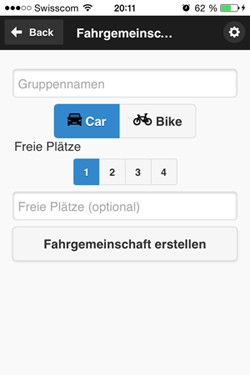
\includegraphics[scale=0.5]{images/app/add_carpool.png}
\caption{Fahrgemeinschaft erstellen}
\label{fig:app_add_carpool}
\end{figure}


\newpage
\FloatBarrier
\subsubsection{Resultate}
Unter Resultate (siehe Abbildung \ref{fig:app_results}) finden angemeldete Benutzer ihre Bestleistungen und die letzten Resultate.
\begin{figure}[h]
\centering
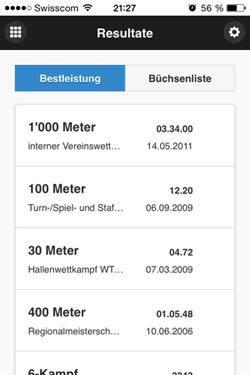
\includegraphics[scale=0.5]{images/app/results.png}
\caption{Resultate Seite}
\label{fig:app_results}
\end{figure}


\FloatBarrier
\subsubsection{Einstellungen}
In den Einstellungen kann sich der Benutzer nicht nur einloggen (siehe Abbildung \ref{fig:app_login}), sondern auch wählen, für welche Riege er die Matches, Anlässe und Trainings sehen möchte (siehe Abbildung \ref{fig:app_riege_setting}). Diese Filter werden dann auf die Veranstaltungsübersichtseiten angewendet.
\begin{figure}[ht]
\centering
\subfigure[Login Formular]{
  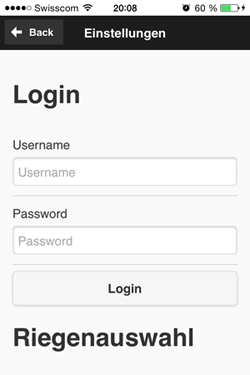
\includegraphics[scale=0.5]{images/app/settings1.png}
  \label{fig:app_login}
}
\subfigure[Riegen Einstellungen]{
  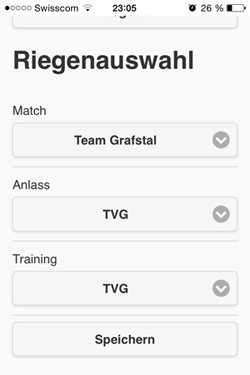
\includegraphics[scale=0.5]{images/app/settings2.png}
  \label{fig:app_riege_setting}
}
\label{fig:app_settings}
\caption{Einstellungen}
\end{figure}

\newpage
\FloatBarrier
\subsection{Javascript Funktionen}
Die Javascript Funktionen wurden möglichst generisch gewählt, damit man sie an verschiedenen Orten wiederverwenden kann. Mit diesem Ansatz ist man bei den verschiedenen Veranstaltungsseiten mit wenig Code ausgekommen. Es war auch einfach, die nächste bevorstehende Veranstaltung auf der Startseite gleich anzuzeigen, wie auf den anderen Seiten. Das App kommt durch das mit knapp 2'000 Zeilen Code aus. Die Funktionen wurden in unterschiedliche Files geschrieben, welche nach ihrem Zweck benannt wurden.
\begin{itemize}
\item carpool.js: an- und abmelden bei Fahrgemeinschaften, anzeigen von Fahrgemeinschaften
\item help.js:  Datum formatieren,  Listen-Elemente erstellen, Navigationselemente
\item index.js: initialisieren der Push-Benachrichtigungen
\item news.js: Berichte laden
\item result.js: Resultate anzeigen
\item settings.js: Dropwdowns initialisieren, an- und abmelden, Riegenfilter setzen
\item signinObject.js: Veranstaltungen laden, Veranstaltungsdetails anzeigen, an- und abmelden bei Veranstaltungen 
\end{itemize}

\subsection{Login}
Da das Backend nur über eine HTTP-Verbindung verfügte und die Anmeldedaten nicht im localStorage  gespeichert werden sollten, wurde darauf verzichtet, die Anmeldedaten bei jeder Anfrage an das Backend mitzusenden. Bei der Anmeldung wird die Mitglieder-ID gespeichert und bei einer Anfrage mitgeteilt. In einem späteren Projekt sollte diese Lösung durch eine Session-ID abgelöst werden.

\subsection{Provisioning Prozesse}
Die Entwicklung der App ist das eine, die Bereitstellung zum Download das andere. Phonegap hilft beim Provisioning vor allem bei Android. Es erstellt, richtig konfiguriert, ein signiertes APK-Paket, welches in der Google Play Developer Console hochgeladen werden kann. Zuerst muss man jedoch einen Developer Account eröffnen. Anschliessend kann man die Beschreibung und die Screenshots für die App hochladen. Das ganze dauert nur wenige Minuten, eine Stunde nach dem Absenden findet man seine App in Google Play. Es empfiehlt sich, die App noch mit eine Absender-ID zu verknüpfen, damit man Statistiken über die Downloadzahlen ansehen kann. (siehe dazu auch \cite{android_prov})

Bei Apple sieht das etwas anders aus: Phonegap kann kein Paket erstellen, es erstellt lediglich das Projekt. Das Projekt muss man dann in XCode öffnen und von dort aus das eigentliche Paket erstellen. Auch hier benötigt man einen Developer Account, den man wahrscheinlich bereits besitzt, da man ihn zum Testen auf realen Geräten benötigt. Zusätzlich muss man ein Distribution Certificate erstellen und in XCode hinzufügen. Danach muss man in iTunes Connect noch einige Angaben zu den Inhalten der App machen. Des Weiteren muss man Review Informationen bereitstellen, dass heisst einen Test Benutzer und Informationen zur Entwicklung angeben. Erst wenn die App erfasst wurde, kann man in XCode ein Archiv erstellen und dieses direkt zu iTunes Connect hochladen. Nun werden schon die ersten Tests durchgeführt, ob zum Beispiel die Versionsnummern übereinstimmen und ob für jedes unterstütze Gerät Screenshots erfasst wurden. Falls dies nicht der Fall ist, wird die App abgelehnt und man muss die Dinge beheben. An diesem Punkt beginnt das Warten - die durchschnittliche Review-Zeit beträgt 8 Tage. (siehe dazu auch \cite{apple_prov_apple} und \cite{apple_prov_ralf})

\subsection{Probleme}
Die Entwicklung für verschiedenen Plattformen war nicht immer einfach. Es kann zwar der gleiche Code verwendet werden, jedoch wird dieser zum Teil anders interpretiert. Bei iOS stellte zum Beispiel die Datum Konvertierung von Daten aus PHP in Javascript ein Problem dar Die Daten mussten aufgesplittet werden und in Javascript ein neues Datum Objekt mit den einzelnen Teilen erstellt werden. Des Weiteren wurde unter Android der Löschaufruf für Fahrgemeinschaften gepuffert. Die App zeigte zwar an, dass die Fahrgemeinschaft gelöscht worden sei, doch es wurde nie ein Löschauftrag an das Backend geschickt. Dieser Fehler wurde bei jQuery raportiert (siehe \cite{bug_jquery}) und mittels eines Workarounds umgangen. Ein weiterer Fehler (siehe \cite{bug_jquery_mobile}) wurde in jQuery Mobile gefunden, es gab hier Probleme mit der Navigation, wenn die grafischen Übergange von jQuery Mobile abgeschaltet wurden. Dieser Fehler konnte jedoch auch mit einem Workaround umgangen werden.
